\documentclass[11pt, oneside]{article}   	% use "amsart" instead of "article" for AMSLaTeX format
\usepackage{geometry}                		% See geometry.pdf to learn the layout options. There are lots.
\geometry{letterpaper}                   		% ... or a4paper or a5paper or ... 
%\geometry{landscape}                		% Activate for for rotated page geometry
%\usepackage[parfill]{parskip}    		% Activate to begin paragraphs with an empty line rather than an indent
\usepackage{graphicx}				% Use pdf, png, jpg, or eps� with pdflatex; use eps in DVI mode
								% TeX will automatically convert eps --> pdf in pdflatex		
\usepackage{amssymb}
\usepackage{amsmath}
\usepackage{parskip}
\usepackage{color}

\title{Uniform Circular Motion}
%\author{The Author}
%\section{}
% \subsection*{R code}
\date{}							% Activate to display a given date or no date

\graphicspath{{/Users/telliott_admin/Dropbox/Tex/png/}}

% \begin{center} 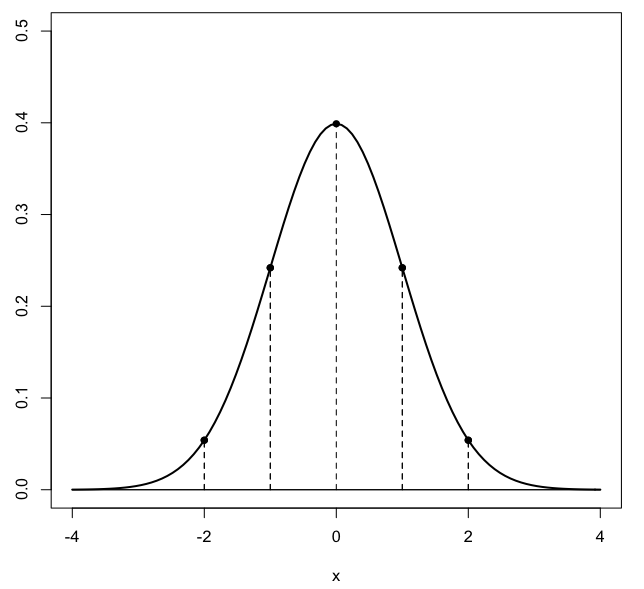
\includegraphics [scale=0.4] {gauss3.png} \end{center}

\begin{document}
\maketitle
\Large
\noindent
Here we want to think about some problems related to the orbits of planets.  Perhaps the first issue to deal with is uniform circular motion.  In this analysis we will idealize the orbits of the planets as circles.

According to wikipedia, the eccentricity of an ellipse is 
\[ e = \sqrt{1 - (\frac{b^2}{a^2})} = \frac{f}{a} \]
where $f = \sqrt{a^2 - b^2}$ is the distance from the center to either focus.
(need to prove this)

Also according to wikipedia, the eccentricity of orbit of the planets known to Kepler plus the moon are
\[ 
\begin{array}{lcr}
\mbox{Mercury} & 0.024  \\
\mbox{Venus} & 0.007  \\
\mbox{Earth} & 0.017  \\
\mbox{Mars} & 0.093  \\
\mbox{Jupiter} & 0.048  \\
\mbox{Saturn} & 0.054  \\
\mbox{Moon} & 0.055  \\
\end{array}
\] 
So looking at Earth, for example, its mean distance from the sun is 150 million kilometers, so approximating $a$ as that value, $f=ea$ is about 2.5 in the same units.  The radius of the sun is about 0.7 in those units.
(Need to re-check this calculation because it disagrees with result based on center of mass).

\subsection*{basic equations}
We're quite familiar with polar coordinates, we write
\[ x = R \cos \theta \]
\[ y = R \sin \theta \]
(I'm going to use $R$ for the radius since we will also have $\mathbf{r}(t)$, the position vector).

We are talking about objects that change position with time, so we need to introduce time here somehow.  We will say that 
\[ \theta = \omega t \]
Our clock ticks, and $\omega$ (in units of radians per second) tells how $\theta$ is calibrated with respect to the clock.

So now we can write the components of 
\[ \mathbf{r}(t) = \langle \ x(t), y(t) \ \rangle \]
\[ \mathbf{r}(t) = R \langle \cos \theta, \sin \theta \rangle \]
\[ \mathbf{r}(t) = R \langle \cos \omega t, \sin \omega t \rangle \]
And then we just differentiate to find the velocity and acceleration
\[ \mathbf{v}(t) = \omega R \langle -\sin \omega t, \cos \omega t \rangle \]
\[ \mathbf{a}(t) = -\omega^2 R \langle \cos \omega t, \sin \omega t \rangle \]
\[ \mathbf{a}(t) = -\omega^2 R \mathbf{r}(t) \]
Notice that $\mathbf{v}(t)$ is orthogonal to $\mathbf{r}(t)$
\begin{center} 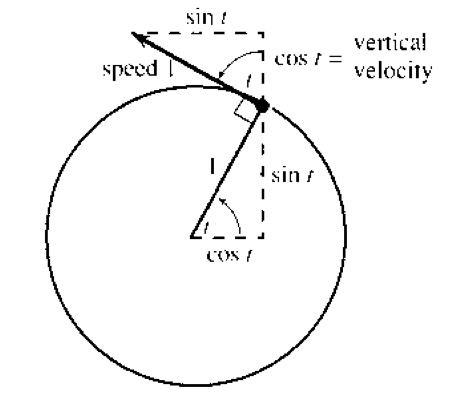
\includegraphics [scale=0.6] {strang_ucm.png} \end{center}
\[ \mathbf{v}(t) \cdot \mathbf{r}(t) = 0 \]
and the acceleration is on exactly the same line as $\mathbf{r}$ but points inward, toward the sun or origin of the system.
\[ \mathbf{a}(t) = -\omega^2 R \mathbf{r}(t) \]
Perhaps if we adjusted our clock to have the appropriate units of time, we wouldn't need $\omega$, but it gives the magnitude of the velocity.
\[ v = |\mathbf{v}| = \omega R  \]
\[ a = |\mathbf{a}| = \omega^2 R \]
so
\[ a =  \omega^2 R = (\frac{v}{R})^2 R = \frac{v^2}{R} \]
We can apply the formula to find the orbital velocity for an object going around the earth.  The acceleration is due to gravity so
\[ \mathbf{F} = m \mathbf{a} \]
Its magnitude is 
\[ a = \frac{GM}{R^2} = \frac{v^2}{R} \]
So
\[ v = \sqrt{\frac{GM}{R}} \]
For the earth
\[ 
\begin{array}{lcr}
\mbox{G =} & 6.67384 \times 10^{-11} \ \text{m}^3 \ \text{kg}^{-1} \ \text{s}^{-2}  \\
\mbox{R =} & 6.371 \times 10^{6} \ \text{m}  \\
\mbox{M =} & 5.97219 \times 10^24 \ \text{kg}  \\
\end{array}
\] 
so $GM/R \approx 6.26 \times 10^7$ and $v \approx 7910$ m/s.  If we increase $R$ to an height of $150$ km above the surface of the earth we would have $v \approx 7815$ m/s.  

Also, we can compare these numbers with the velocity of rotation at the earth's surface.  Roughly speaking, the circumference of the earth is $25,000$ miles ($24,908$ miles, $40,075$ km) and it rotates in $24$ hr, so the speed is about $1037$ mph.  That is about $463$ m/s$^2$.  

Of course, the velocity depends on latitude.  One must multiply by the cosine of the latitude.

In addition we need to add the potential energy to get to a particular orbit.   We have
\[ V = - GM/R \]
\[ \Delta V = -GM(\frac{1}{R_2} - \frac{1}{R_1}) = GM(\frac{1}{R_1} - \frac{1}{R_2})\]
We can use these to look at some other orbits.
Geostationary orbit  42,000 km
Moon orbit avg = 385,000 km

The variation in satellite orbits is pretty extreme.
\subsection*{energy}
The force due to gravity is
\[ \mathbf{F} = -\frac{GmM}{r^2} \hat{\mathbf{r}} \]
The potential is a function, which when we take
\[ - \frac{d}{dr} U = \mathbf{F} \]
\[ U = - \frac{GmM}{r} + C \]
Define
\[ U_{\infty} = 0 \rightarrow C = 0 \]
The total energy is
\[ E = K + U = \frac{1}{2}mv^2 - \frac{GmM}{r} \]
if we want an object to just reach $r=\infty$ with zero energy, then
\[ 0 = \frac{1}{2}mv^2 - \frac{GmM}{r} \]
\[ v^2 = \frac{2GM}{r} \]
This is the escape velocity.

If the force is as given above, the magnitude of the acceleration is 
\[ a = \frac{GM}{r^2} \]
but for uniform circular motion we had
\[ a = \frac{v^2}{r} = \frac{GM}{r^2} \]
\[ v^2 = \frac{GM}{r} \]
This is the orbital velocity.

Finally, we know that the velocity is distance divided by time, so for one full revolution it is
\[ v = \frac{2\pi r}{T} \]
but
\[ v^2 = \frac{GM}{r} = (\frac{2\pi r}{T})^2 \]
Rearranging
\[ T^2 = \frac{(2\pi)^2}{GM} r^3 \]
This is Kepler's Third Law.  The derivation is easy if we assume the orbits are circles, which is pretty close to being true.  It is also true for an elliptical orbit.  That is a bit harder calculation, which I have written up elsewhere.

\end{document}  